%%% api - arquitetura
\begin{frame}{Aplicação \textit{web} - Funcionalidades}

\vspace*{-3em}

\begin{itemize}
	\item Possibilitar autenticação por parte de organizações;
	\item permitir edição do perfil da organização autenticada e interação da mesma com a plataforma;
	\item disponibilizar contacto de voluntários interessados num evento.	
\end{itemize}

\end{frame}

%%% api - arquitetura
\begin{frame}{Aplicação \textit{web} - Arquitetura}
	
\vspace*{-3em}
	
\begin{itemize}
	\item \textbf{Classe Principal}: instancia serviços da API e define roteamento da aplicação;
	\item \textbf{Componentes}: definem a interface de utilizador, incluindo o tratamento de operações de \textit{input};
	\item \textbf{API}: contém implementação de serviços utilizados para aceder à \textit{web} API.
\end{itemize}		

\centering
\scalebox{0.4}{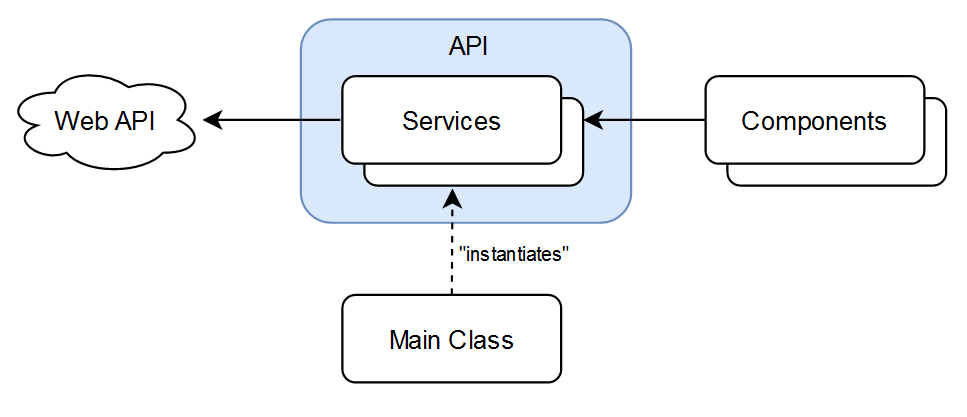
\includegraphics{Figures/web_app_architecture}}\\

{\small Arquitetura da aplicação \textit{web}.}

\end{frame}